% Options for packages loaded elsewhere
\PassOptionsToPackage{unicode}{hyperref}
\PassOptionsToPackage{hyphens}{url}
%
\documentclass[
]{book}
\usepackage{amsmath,amssymb}
\usepackage{lmodern}
\usepackage{iftex}
\ifPDFTeX
  \usepackage[T1]{fontenc}
  \usepackage[utf8]{inputenc}
  \usepackage{textcomp} % provide euro and other symbols
\else % if luatex or xetex
  \usepackage{unicode-math}
  \defaultfontfeatures{Scale=MatchLowercase}
  \defaultfontfeatures[\rmfamily]{Ligatures=TeX,Scale=1}
\fi
% Use upquote if available, for straight quotes in verbatim environments
\IfFileExists{upquote.sty}{\usepackage{upquote}}{}
\IfFileExists{microtype.sty}{% use microtype if available
  \usepackage[]{microtype}
  \UseMicrotypeSet[protrusion]{basicmath} % disable protrusion for tt fonts
}{}
\makeatletter
\@ifundefined{KOMAClassName}{% if non-KOMA class
  \IfFileExists{parskip.sty}{%
    \usepackage{parskip}
  }{% else
    \setlength{\parindent}{0pt}
    \setlength{\parskip}{6pt plus 2pt minus 1pt}}
}{% if KOMA class
  \KOMAoptions{parskip=half}}
\makeatother
\usepackage{xcolor}
\IfFileExists{xurl.sty}{\usepackage{xurl}}{} % add URL line breaks if available
\IfFileExists{bookmark.sty}{\usepackage{bookmark}}{\usepackage{hyperref}}
\hypersetup{
  pdftitle={A primer in Human Cardiovascular Genetics},
  pdfauthor={dr. Sander W. van der Laan \textbar{} swvanderlaan},
  hidelinks,
  pdfcreator={LaTeX via pandoc}}
\urlstyle{same} % disable monospaced font for URLs
\usepackage{color}
\usepackage{fancyvrb}
\newcommand{\VerbBar}{|}
\newcommand{\VERB}{\Verb[commandchars=\\\{\}]}
\DefineVerbatimEnvironment{Highlighting}{Verbatim}{commandchars=\\\{\}}
% Add ',fontsize=\small' for more characters per line
\usepackage{framed}
\definecolor{shadecolor}{RGB}{248,248,248}
\newenvironment{Shaded}{\begin{snugshade}}{\end{snugshade}}
\newcommand{\AlertTok}[1]{\textcolor[rgb]{0.94,0.16,0.16}{#1}}
\newcommand{\AnnotationTok}[1]{\textcolor[rgb]{0.56,0.35,0.01}{\textbf{\textit{#1}}}}
\newcommand{\AttributeTok}[1]{\textcolor[rgb]{0.77,0.63,0.00}{#1}}
\newcommand{\BaseNTok}[1]{\textcolor[rgb]{0.00,0.00,0.81}{#1}}
\newcommand{\BuiltInTok}[1]{#1}
\newcommand{\CharTok}[1]{\textcolor[rgb]{0.31,0.60,0.02}{#1}}
\newcommand{\CommentTok}[1]{\textcolor[rgb]{0.56,0.35,0.01}{\textit{#1}}}
\newcommand{\CommentVarTok}[1]{\textcolor[rgb]{0.56,0.35,0.01}{\textbf{\textit{#1}}}}
\newcommand{\ConstantTok}[1]{\textcolor[rgb]{0.00,0.00,0.00}{#1}}
\newcommand{\ControlFlowTok}[1]{\textcolor[rgb]{0.13,0.29,0.53}{\textbf{#1}}}
\newcommand{\DataTypeTok}[1]{\textcolor[rgb]{0.13,0.29,0.53}{#1}}
\newcommand{\DecValTok}[1]{\textcolor[rgb]{0.00,0.00,0.81}{#1}}
\newcommand{\DocumentationTok}[1]{\textcolor[rgb]{0.56,0.35,0.01}{\textbf{\textit{#1}}}}
\newcommand{\ErrorTok}[1]{\textcolor[rgb]{0.64,0.00,0.00}{\textbf{#1}}}
\newcommand{\ExtensionTok}[1]{#1}
\newcommand{\FloatTok}[1]{\textcolor[rgb]{0.00,0.00,0.81}{#1}}
\newcommand{\FunctionTok}[1]{\textcolor[rgb]{0.00,0.00,0.00}{#1}}
\newcommand{\ImportTok}[1]{#1}
\newcommand{\InformationTok}[1]{\textcolor[rgb]{0.56,0.35,0.01}{\textbf{\textit{#1}}}}
\newcommand{\KeywordTok}[1]{\textcolor[rgb]{0.13,0.29,0.53}{\textbf{#1}}}
\newcommand{\NormalTok}[1]{#1}
\newcommand{\OperatorTok}[1]{\textcolor[rgb]{0.81,0.36,0.00}{\textbf{#1}}}
\newcommand{\OtherTok}[1]{\textcolor[rgb]{0.56,0.35,0.01}{#1}}
\newcommand{\PreprocessorTok}[1]{\textcolor[rgb]{0.56,0.35,0.01}{\textit{#1}}}
\newcommand{\RegionMarkerTok}[1]{#1}
\newcommand{\SpecialCharTok}[1]{\textcolor[rgb]{0.00,0.00,0.00}{#1}}
\newcommand{\SpecialStringTok}[1]{\textcolor[rgb]{0.31,0.60,0.02}{#1}}
\newcommand{\StringTok}[1]{\textcolor[rgb]{0.31,0.60,0.02}{#1}}
\newcommand{\VariableTok}[1]{\textcolor[rgb]{0.00,0.00,0.00}{#1}}
\newcommand{\VerbatimStringTok}[1]{\textcolor[rgb]{0.31,0.60,0.02}{#1}}
\newcommand{\WarningTok}[1]{\textcolor[rgb]{0.56,0.35,0.01}{\textbf{\textit{#1}}}}
\usepackage{longtable,booktabs,array}
\usepackage{calc} % for calculating minipage widths
% Correct order of tables after \paragraph or \subparagraph
\usepackage{etoolbox}
\makeatletter
\patchcmd\longtable{\par}{\if@noskipsec\mbox{}\fi\par}{}{}
\makeatother
% Allow footnotes in longtable head/foot
\IfFileExists{footnotehyper.sty}{\usepackage{footnotehyper}}{\usepackage{footnote}}
\makesavenoteenv{longtable}
\usepackage{graphicx}
\makeatletter
\def\maxwidth{\ifdim\Gin@nat@width>\linewidth\linewidth\else\Gin@nat@width\fi}
\def\maxheight{\ifdim\Gin@nat@height>\textheight\textheight\else\Gin@nat@height\fi}
\makeatother
% Scale images if necessary, so that they will not overflow the page
% margins by default, and it is still possible to overwrite the defaults
% using explicit options in \includegraphics[width, height, ...]{}
\setkeys{Gin}{width=\maxwidth,height=\maxheight,keepaspectratio}
% Set default figure placement to htbp
\makeatletter
\def\fps@figure{htbp}
\makeatother
\setlength{\emergencystretch}{3em} % prevent overfull lines
\providecommand{\tightlist}{%
  \setlength{\itemsep}{0pt}\setlength{\parskip}{0pt}}
\setcounter{secnumdepth}{5}
\usepackage{booktabs}
\usepackage{amsthm}
\makeatletter
\def\thm@space@setup{%
  \thm@preskip=8pt plus 2pt minus 4pt
  \thm@postskip=\thm@preskip
}
\makeatother
\ifLuaTeX
  \usepackage{selnolig}  % disable illegal ligatures
\fi
\usepackage[]{natbib}
\bibliographystyle{apalike}

\title{A primer in Human Cardiovascular Genetics}
\author{\href{https://swvanderlaan.github.iio}{dr. Sander W. van der Laan} \textbar{} \href{https://www.twitter.com/swvanderlaan}{swvanderlaan}}
\date{Last update: 2022-03-24}

\begin{document}
\maketitle

{
\setcounter{tocdepth}{1}
\tableofcontents
}
\hypertarget{about-this-primer}{%
\chapter{About this primer}\label{about-this-primer}}

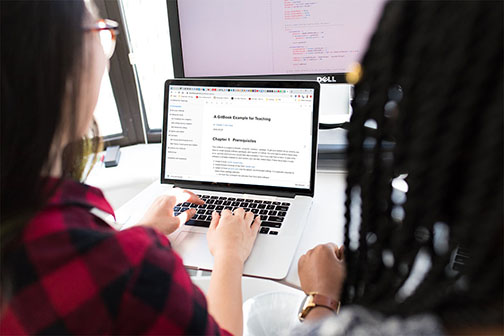
\includegraphics{./img/using_gitbook.jpeg}

\hypertarget{introduction}{%
\section{Introduction}\label{introduction}}

Welcome to the \emph{A primer in Human Cardiovascular Genetics} as part of the \textbf{Genetic Epidemiology} course. In the next few days we will use this \href{https://cjvanlissa.github.io/gitbook-demo/}{GitBook} to perform quality control (QC), executing a genome-wide association study (GWAS), annotating the GWAS results, and performing further downstream analyses. We will use data from the first release of the \href{https://www.wtccc.org.uk/ccc1/overview.html}{\emph{Welcome Trust Case-Control Consortium (WTCCC)}} and focus on coronary artery disease (CAD).

Unfortunately, during this course there is no time to perform \href{https://www.nature.com/articles/nrg2796}{imputation}, but I will provide some pointers during the course as to how to do this with minimal coding/scripting experience. And I will add a whole chapter on imputation to a future version.

\hypertarget{background-reading}{%
\section{Background reading}\label{background-reading}}

Part of this is based on four great Nature Protocols from the \href{https://www.well.ox.ac.uk/research/research-groups/zondervan-group}{Zondervan group} at the Wellcome Center Human Genetics.

\begin{enumerate}
\def\labelenumi{\arabic{enumi}.}
\tightlist
\item
  \href{https://www.ncbi.nlm.nih.gov/pubmed/17947991}{Zondervan KT \emph{et al.} \emph{Designing candidate gene and genome-wide case-control association studies.} Nat Protoc 2007.}
\item
  \href{https://www.ncbi.nlm.nih.gov/pubmed/19390530}{Pettersson FH \emph{et al.} \emph{Marker selection for genetic case-control association studies.} Nat Protoc 2009.}
\item
  \href{https://www.ncbi.nlm.nih.gov/pubmed/21085122}{Anderson CA \emph{et al.} \emph{Data QC in genetic case-control association studies.} Nat Protoc 2010.}
\item
  \href{https://www.ncbi.nlm.nih.gov/pubmed/21293453}{Clarke GM \emph{et al.} \emph{Basic statistical analysis in genetic case-control studies.} Nat Protoc 2011.}
\end{enumerate}

An update on the community standards of QC for GWAS can be found here:

\begin{enumerate}
\def\labelenumi{\arabic{enumi}.}
\tightlist
\item
  \href{https://www.ncbi.nlm.nih.gov/pubmed/20718045}{Laurie CC \emph{et al.} \emph{Quality control and quality assurance in genotypic data for genome-wide association studies.} Genet Epidemiol 2010.}
\end{enumerate}

With respect to imputation you should also get familiar with the following two works:

\begin{enumerate}
\def\labelenumi{\arabic{enumi}.}
\tightlist
\item
  \href{https://doi.org/10.1038/nrg2796}{Marchini, J. and Howie, B. \emph{Genotype imputation for genome-wide association studies.} Nat Rev Genet 2010}
\item
  \href{https://www.ncbi.nlm.nih.gov/pubmed/18852200}{de Bakker PIW \emph{et al.} \emph{Practical aspects of imputation-driven meta-analysis of genome-wide association studies.} Hum Mol Genet 2008.}
\item
  \href{https://www.ncbi.nlm.nih.gov/pubmed/24762786}{Winkler TW \emph{et al.} \emph{Quality control and conduct of genome-wide association meta-analyses.} Nat Protoc 2014.}
\end{enumerate}

Importantly, follow this practical, but also review the questions asked in the presentation (on the screen or in the Dropbox) and try to answer them.

\hypertarget{meet-the-team}{%
\section{Meet the Team}\label{meet-the-team}}

We work with a team of enthusiastic lecturers with experience in bioinformatics, GWAS, genetic analyses, Mendelian randomization, and epidemiology. This year the team consists of:

\begin{longtable}[]{@{}
  >{\raggedright\arraybackslash}p{(\columnwidth - 0\tabcolsep) * \real{0.2083}}@{}}
\toprule
\endhead
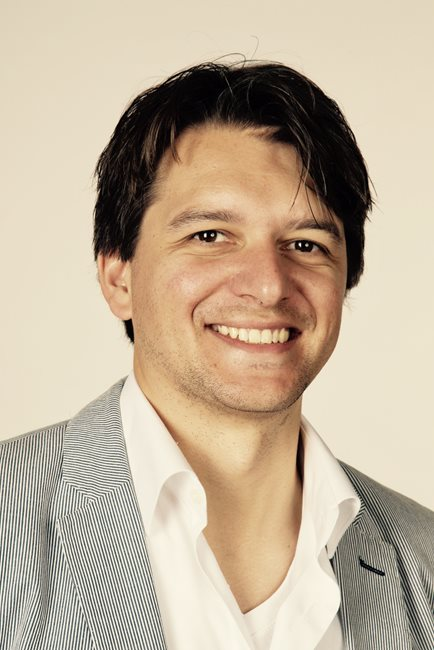
\includegraphics[width=0.15\textwidth,height=\textheight]{img/_team/sander_vander_laan.jpg} Sander W. van der Laan \emph{Assistant professor}Course coordinator\href{mailto:s.w.vanderlaan-2@umcutrecht.nl}{\nolinkurl{s.w.vanderlaan-2@umcutrecht.nl}} \textbar{} \href{http://www.twitter.com/swvanderlaan}{swvanderlaan} \\
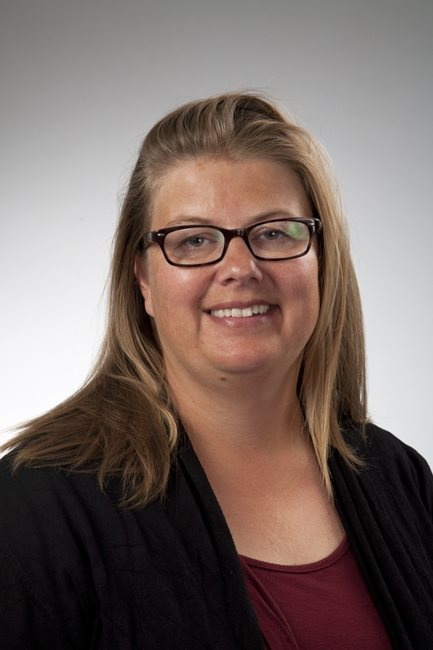
\includegraphics[width=0.15\textwidth,height=\textheight]{img/_team/charlotte_onland.jpg} Charlotte Onland-Moret \emph{Associate Professor}\href{mailto:N.C.Onland@umcutrecht.nl}{\nolinkurl{N.C.Onland@umcutrecht.nl}} \\
\href{img/_team/jessica_van_setten.jpg}{} Jessica van Setten \emph{Assistant professor}\href{mailto:j.vansetten@umcutrecht.nl}{\nolinkurl{j.vansetten@umcutrecht.nl}} \textbar{} \href{http://www.twitter.com/j_vansetten}{j\_vansetten} \\
 \\
 \\
\bottomrule
\end{longtable}

\textbf{Getting started}

Ready to start? Your first point of action is to prepare your system for this course (Chapter \ref{prerequisites}).

\hypertarget{prerequisites}{%
\chapter{Prerequisites}\label{prerequisites}}

\hypertarget{linux-macos-and-windows}{%
\section{Linux, macOS, and Windows}\label{linux-macos-and-windows}}

Most programs made to execute genetic studies are developed for the Unix environment, \emph{e.g.} Linux and macOS. Therefore, they may not work as intended on window's environment. Fortunately, Windows now allow users to install a linux subsystem within Windows 10 and you can find the detail \href{https://docs.microsoft.com/en-us/windows/wsl/about}{guide} here.\\
However, we highly recommend to 1) either install a linux subsystem on your Windows computer (\emph{e.g.} \href{https://blog.storagecraft.com/the-dead-simple-guide-to-installing-a-linux-virtual-machine-on-windows/}{a virtual machine with Ubuntu could work}), or 2) switch to macOS in combination with \href{https://brew.sh}{homebrew} as this will give you advantage of a powerful computer with a userfriendly interface and all the flexibility to use Unix-based programs for your work.

\begin{quote}
For this practical we use a Windows laptop with Ubuntu on a VirtualMachine. Therefore every command is intended for Linux/macOS.
\end{quote}

\hypertarget{programs-you-need}{%
\section{Programs you need}\label{programs-you-need}}

You need few programs for this practical or for your (future) genetic epidemiology work for that matter.

\begin{longtable}[]{@{}
  >{\raggedright\arraybackslash}p{(\columnwidth - 4\tabcolsep) * \real{0.1667}}
  >{\raggedright\arraybackslash}p{(\columnwidth - 4\tabcolsep) * \real{0.1111}}
  >{\raggedright\arraybackslash}p{(\columnwidth - 4\tabcolsep) * \real{0.5694}}@{}}
\toprule
\begin{minipage}[b]{\linewidth}\raggedright
Program
\end{minipage} & \begin{minipage}[b]{\linewidth}\raggedright
Link
\end{minipage} & \begin{minipage}[b]{\linewidth}\raggedright
Description
\end{minipage} \\
\midrule
\endhead
PLINK & {[}\url{https:/} & /www.cog-genomics.org/plink2/{]}(\url{https://www.cog-genomics.org/plink2/})\{target=``\_blank''\} PLINK is a free, open-source genetic analysis toolset, designed to perform a range of basic data parsing and quality control, as well as basic and large-scale analyses in a computationally efficient manner. \\
R & {[}\url{https:/} & /cran.r-project.org{]}(\url{https://cran.r-project.org/})\{target=``\_blank''\} Progam to perform statistical analysis and visualisations. \\
RStudio & {[}\url{https:/} & /www.rstudio.com{]}(\url{https://www.rstudio.com})\{target=``\_blank''\} A userfriendly R-wrap-around for code editing, debugging, analyses, and visualisation \\
\bottomrule
\end{longtable}

Table 1: Programs needed for genetic epidemiology.

All genetic analyses can be done in PLINK, even on your laptop, but with large datasets, e.g.~UK-biobank size, it's better to switch to a \href{https://wiki.bioinformatics.umcutrecht.nl/bin/view/HPC/WebHome}{high-performance computing cluster} like we have at the Uithof.

Nowadays, a lot of people also use programs like \href{snptest}{SNPTEST}, \href{https://data.broadinstitute.org/alkesgroup/BOLT-LMM/}{BOLT-LMM}, and \href{http://cnsgenomics.com/software/gcta/\#Overview}{GCTA} as alternatives to run GWAS and downstream analyses, \emph{e.g.} heritability estimation, Fst-calculation, etc.

Mendelian randomisation can be done either with the \href{http://cnsgenomics.com/software/smr/\#Overview}{SMR} or \href{http://cnsgenomics.com/software/gsmr/}{GSMR} function from GCTA or with R-packages, like \texttt{TwoSampleMR}.

\hypertarget{the-terminal}{%
\section{The Terminal}\label{the-terminal}}

For all the above programs, except RStudio, you will need the \texttt{Terminal}. This comes with every major operating system. And you will (start to) make your own scripts. The benefit of using scripts is that each step is clearly layed out and easily replicable, thus allows for greater reproducibility, easier troubleshooting and can be run on high-performance computer clusters.

Download the data you need to your Desktop: LINK.

Now open the terminal, it should be on the left in the toolbar as a little black computer-monitor-like icon.
Mac uses can type \texttt{command\ +\ space} and type \texttt{terminal}, a terminal screen should open.

\begin{quote}
From now on we will use little code blocks like the example to indicate a code you should type/copy-paste and hit enter. If a code is followed by a comment, it is indicated by a \# - you don't need to copy-paste and execute this.
\end{quote}

\begin{verbatim}
CODE BLOCK

CODE BLOCK # some comment here

\end{verbatim}

You can navigate around the computer through the terminal by typing \texttt{cd\ \textless{}path\textgreater{}}; \texttt{cd} stands for ``change directory'' and means ``some\_file\_directory\_you\_want\_to\_go\_to''.

\begin{verbatim}
# For Linux/macOS Users
cd ~ # will bring you to your home directory
cd ../ # will bring you to the parent directory (up one level) 
cd XXX # will bring you to the XXX directory
\end{verbatim}

Let's navigate to the folder you just downloaded.

\begin{verbatim}
cd ~/Desktop/practical
\end{verbatim}

Let's check out what is inside the directory, by listing (\texttt{ls}) its contents.

\begin{verbatim}
ls -lh

# For Linux/macOS Users
ls -l # shows files as list
ls -lh # shows files as list with human readable format 
ls -lt # shows the files as list sorted by time edited
ls -lS # shows the files as list sorted by size
\end{verbatim}

Adding the flags \texttt{-lh} will get you the contents of a directory in a list (\texttt{-l}) and make the size `human-readable' (\texttt{-h}).

You can also count the number of files.

\begin{verbatim}
ls | wc -l
\end{verbatim}

\hypertarget{installing-some-r-packages}{%
\section{Installing some R packages}\label{installing-some-r-packages}}

I tested this VirtualMachine and everything should be fine, except some libraries weren't there. We need to install them.

To be able to install certain \texttt{r}-packages, we need to install some Linux (Ubuntu) software. Type the following:

\begin{verbatim}
sudo apt-get install libcurl4 libcurl4-openssl-dev -y

sudo apt-get install libssl-dev
\end{verbatim}

Now close the terminal window - really making sure that the terminal-program has quit.

Open a new terminal window and open \texttt{r} by simply typing \texttt{R}. You should install the following packages, and then you're good to go!

\begin{verbatim}
install.packages(c("httr", "usethis", "data.table", "devtools", "qqman", "CMplot", "tibble", "plotly", "dplyr"))

library(c("httr", "usethis", "data.table", "devtools", "qqman", "CMplot", "tibble", "plotly", "dplyr"))
devtools::install_github("kassambara/ggpubr")
library("ggpubr")
\end{verbatim}

All in all this may take some time, good moment to relax, review your notes, stretch your legs, or take a coffee.

\hypertarget{getgitbook}{%
\chapter{Get your GitBook}\label{getgitbook}}

To get your GitBook, you should follow these steps:

\begin{enumerate}
\def\labelenumi{\arabic{enumi}.}
\tightlist
\item
  Go to \url{https://github.com/cjvanlissa/gitbook-demo}
\item
  In the top right of the page, click \texttt{Fork}.\\
  This will copy my \texttt{gitbook-demo} repository to your GitHub account.\\
  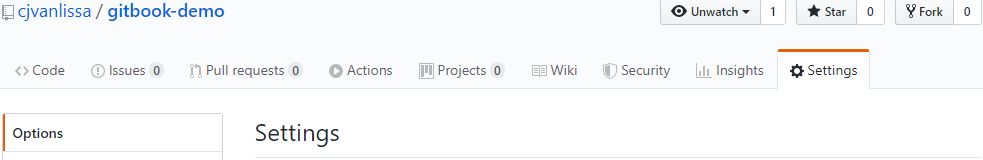
\includegraphics{./img/settings.png}
\item
  My repository is now copied to your account. It is a template repository, which means that you can create a \emph{new repository} based on this one.
\item
  Create a new repository for your own GitBook. Create one for a course you've been wanting to update. In the top-right corner of the GitHub website, click the + icon, and select ``New repository'':\\
  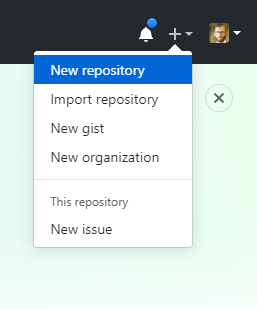
\includegraphics{./img/new_repo.png}
\item
  In the dialog, select the \texttt{gitbook-demo} as ``Repository template'', and give the repository an appropriate name for your course. Then, press \texttt{Create\ repository}:\\
  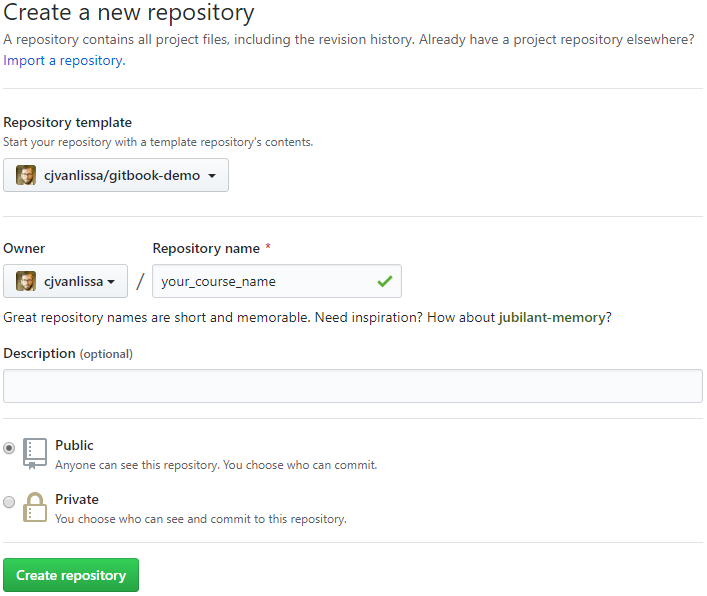
\includegraphics{./img/from_template.png}
\item
  Now, go back to Rstudio on your computer. In Rstudio, click \texttt{File\ \textgreater{}\ New\ Project}. A dialog will open. If you set up Rstudio with Git correctly, the dialog should have an option to create a new project from Version control. Click it:\\
  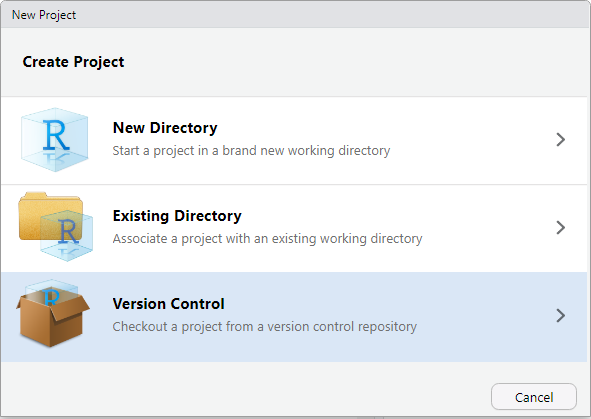
\includegraphics{./img/new_project.png}
\item
  In the next dialog window, you should copy the URL of the GitHub repository you created in \emph{Step 5}, like so:\\
  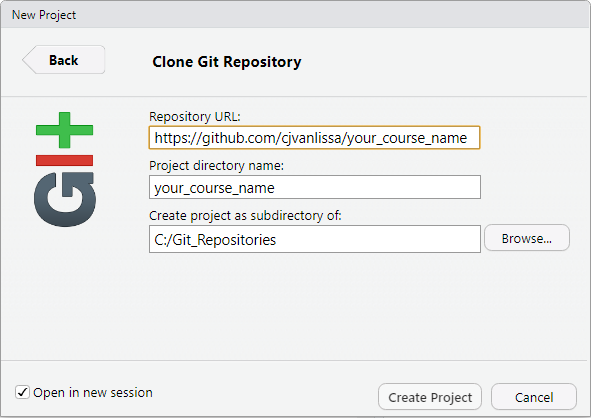
\includegraphics{./img/new_git_project.png}
\item
  Now, in Rstudio, you can open files for editing and create new files (explained in the next Chapter). Open files by clicking them in the Files editor (usually in the bottom right of Rstudio):\\
  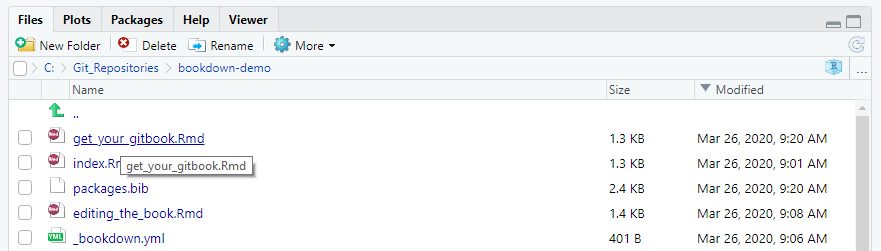
\includegraphics{./img/files_editor.png}
\item
  After you make a change, it will show up in the Git tab (usually in the top right of Rstudio). You must Commit the change locally, and then Push the change to GitHub to update your repo. To Commit, select the file and click the Commit button. Write a short message to describe the changes you made, then click the Commit button again. Now, press Push to send your commits to GitHub.\\
  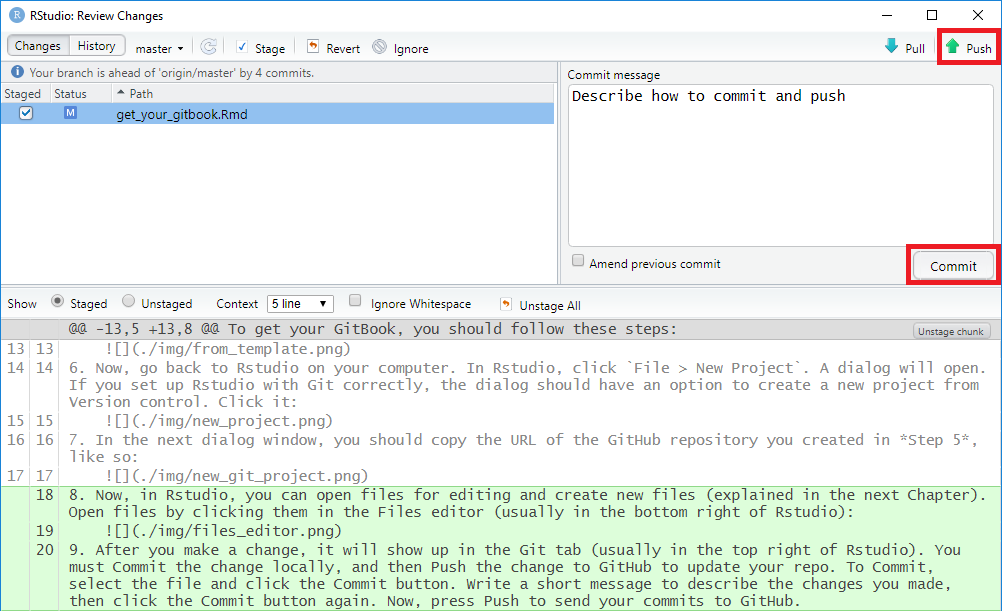
\includegraphics{./img/commit_push.png}
\item
  To render your book as a GitBook, you must ``Build'' it. In the top-right panel of Rstudio, you see a ``Build'' tab. In this tab, simply click the ``Build Book'' button to build your book. You should see a lot of rendering messages, until a window pops up with your brand new GitBook. If you get errors at this stage, you probably made a mistake in preparing your system (see the previous Chapter).\\
  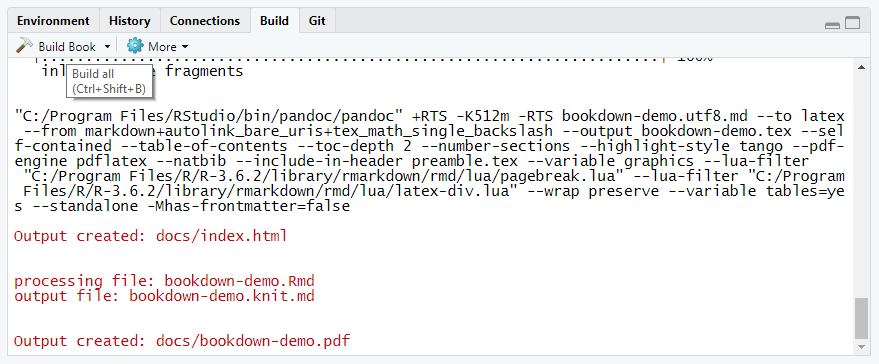
\includegraphics{./img/build_book.png}
\item
  Building the book generated a lot of new files in the \texttt{./docs} directory. This directory contains the website files for your GitBook. Open the Git tab again, verify that the \texttt{./docs} directory is listed, and Commit and Push all of these new files as described in \emph{Step 9}.
\item
  There is only one last remaining task: To publish your GitBook on GitHub pages. Once you do this, any change to the \texttt{./docs} folder that you push to GitHub will lead to an immediate update of your GitBook website. Go back to the GitHub page for your Repository. Click on the \texttt{Settings} tab on the top right of the page:\\
  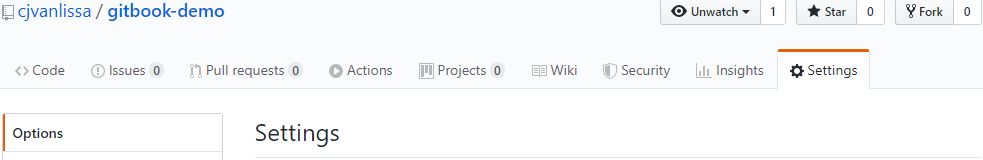
\includegraphics{./img/settings.png}
\item
  On the Settings page, scroll all the way down until you reach a section called \texttt{GitHub\ Pages}. There, under the ``Source'' heading, click the word \texttt{None}, and select \texttt{master\ branch\ /docs\ folder}. When you select it, the page will update, and if you scroll back down to the \texttt{GitHub\ Pages} section, you will see the URL where your GitBook is published. The first time, it will take a few minutes for your GitBook to come online. When you publish updates to the GitBook however (simply by following \emph{Step 11} again), the update will be near-instantaneous. The Pages section should now look like this (and that is hopefully the link where you found this book):\\
  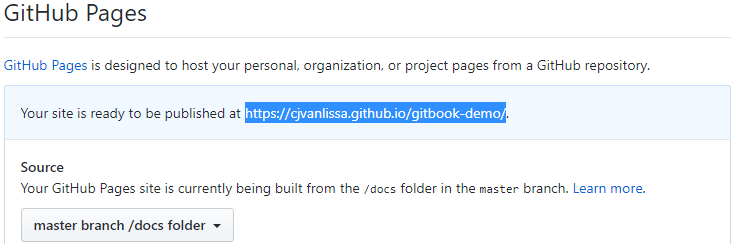
\includegraphics{./img/pages_published.png}
\end{enumerate}

\hypertarget{editing-the-book}{%
\chapter{Editing the book}\label{editing-the-book}}

The contents of the book are written in \textbf{RMarkdown}. You can use any formatting code that Pandoc's Markdown supports, e.g., a math equation \(a^2 + b^2 = c^2\). Moreover, you can include chunks of R-code, like this:

The results of these chunks can be rendered to the GitBook:

\begin{verbatim}
## [1] "This is an R-command!"
\end{verbatim}

To edit the book, you can change the text in the \texttt{.Rmd} files. Each Rmd file should contain \textbf{one and only one} chapter. A chapter is defined by the first-level heading \texttt{\#}, e.g., \texttt{\#\ Editing\ the\ book}.

Any sub-headings within the chapter are indicated with several \texttt{\#} signs, e.g., \texttt{\#\#} (level 2) and \texttt{\#\#\#} (level 3).

\hypertarget{creating-new-chapters}{%
\section{Creating new chapters}\label{creating-new-chapters}}

To create a new chapter, you must follow two steps: 1) Create the file, and 2) Include it in the list of chapters.

First, to create the file for a new chapter in Rstudio, click \texttt{File\ \textgreater{}\ New\ File\ \textgreater{}\ Text\ file}. At the top of the file, write your chapter heading, as explained above. Then, click \texttt{File\ \textgreater{}\ Save}. Save the file as \texttt{.Rmd}, without spaces in the file name, e.g.: \texttt{editing\_the\_book.Rmd}.

Second, to include it in the list of chapters, open the file \texttt{\_bookdown.yml} (click it in the Files explorer in the bottom right of Rstudio). This file has a list of \texttt{.Rmd} files to be included in the book. In this example, the list looks like this:

\begin{Shaded}
\begin{Highlighting}[]
\NormalTok{tmp }\OtherTok{\textless{}{-}} \FunctionTok{readLines}\NormalTok{(}\StringTok{"\_bookdown.yml"}\NormalTok{)}
\FunctionTok{cat}\NormalTok{(tmp[}\FunctionTok{grep}\NormalTok{(}\StringTok{"\^{}rmd\_files"}\NormalTok{, tmp)}\SpecialCharTok{:}\FunctionTok{grep}\NormalTok{(}\StringTok{"references}\SpecialCharTok{\textbackslash{}\textbackslash{}}\StringTok{.Rmd"}\NormalTok{, tmp)], }\AttributeTok{sep =} \StringTok{"}\SpecialCharTok{\textbackslash{}n}\StringTok{"}\NormalTok{)}
\end{Highlighting}
\end{Shaded}

rmd\_files: {[}``index.Rmd'',
``prerequisites.Rmd'',
``get\_your\_gitbook.Rmd'',
``editing\_the\_book.Rmd'',
``figures\_tables.Rmd'',
``examples.Rmd'',
``open\_educational.Rmd'',
``use\_in\_course.Rmd'',
``licenses.Rmd'',
``references.Rmd''{]}

Insert the file name of your new chapter in the desired position in this list.

\hypertarget{linking-across-chapters}{%
\section{Linking across chapters}\label{linking-across-chapters}}

You can label chapter and section titles using \texttt{\{\#label\}} after them. The labels can be used as cross-references. For example, we can link to Chapter \ref{figtab}. If you do not manually label chapters, there will be automatic labels anyway, e.g., Chapter \ref{examples}.

\hypertarget{advanced-editing}{%
\section{Advanced editing}\label{advanced-editing}}

The convenient \href{https://rstudio.com/wp-content/uploads/2016/03/rmarkdown-cheatsheet-2.0.pdf}{Rmarkdown Cheat Sheet} by Rstudio covers most of the knowledge required for advanced Rmarkdown editing. You can print it out and stick it to your wall!

\hypertarget{figtab}{%
\chapter{Figures and tables}\label{figtab}}

Figures and tables with captions will be placed in \texttt{figure} and \texttt{table} environments, respectively.

\begin{Shaded}
\begin{Highlighting}[]
\FunctionTok{par}\NormalTok{(}\AttributeTok{mar =} \FunctionTok{c}\NormalTok{(}\DecValTok{4}\NormalTok{, }\DecValTok{4}\NormalTok{, .}\DecValTok{1}\NormalTok{, .}\DecValTok{1}\NormalTok{))}
\FunctionTok{plot}\NormalTok{(pressure, }\AttributeTok{type =} \StringTok{\textquotesingle{}b\textquotesingle{}}\NormalTok{, }\AttributeTok{pch =} \DecValTok{19}\NormalTok{)}
\end{Highlighting}
\end{Shaded}

\begin{figure}

{\centering 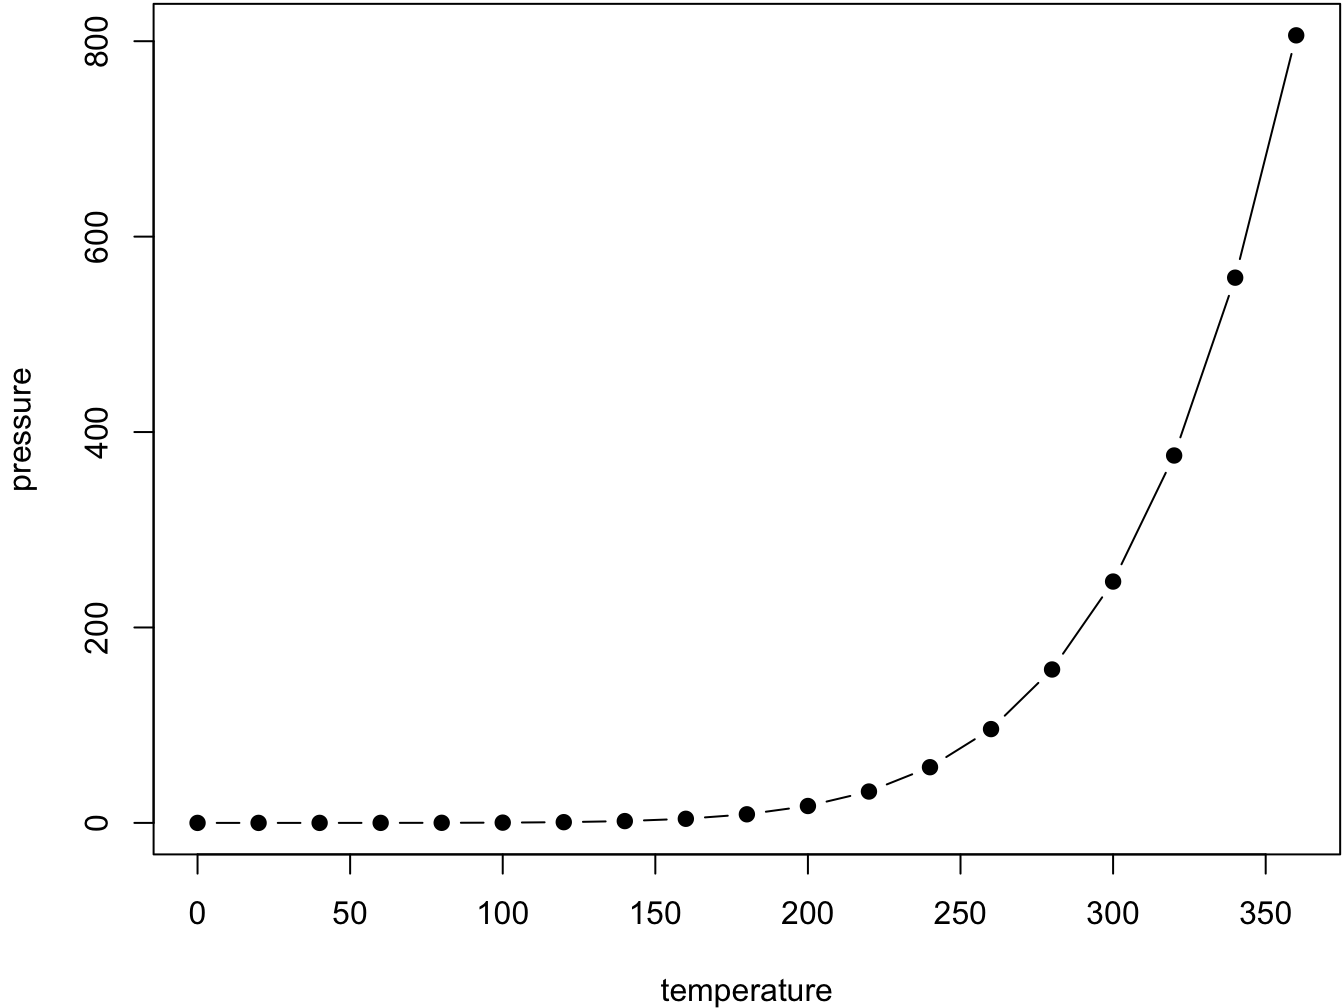
\includegraphics[width=0.8\linewidth]{A-primer-in-Human-Cardiovascular-Genetics_files/figure-latex/nice-fig-1} 

}

\caption{Here is a nice figure!}\label{fig:nice-fig}
\end{figure}

Reference a figure by its code chunk label with the \texttt{fig:} prefix, e.g., see Figure \ref{fig:nice-fig}. Similarly, you can reference tables generated from \texttt{knitr::kable()}, e.g., see Table \ref{tab:nice-tab}.

\begin{Shaded}
\begin{Highlighting}[]
\NormalTok{knitr}\SpecialCharTok{::}\FunctionTok{kable}\NormalTok{(}
  \FunctionTok{head}\NormalTok{(iris, }\DecValTok{20}\NormalTok{), }\AttributeTok{caption =} \StringTok{\textquotesingle{}Here is a nice table!\textquotesingle{}}\NormalTok{,}
  \AttributeTok{booktabs =} \ConstantTok{TRUE}
\NormalTok{)}
\end{Highlighting}
\end{Shaded}

\begin{table}

\caption{\label{tab:nice-tab}Here is a nice table!}
\centering
\begin{tabular}[t]{rrrrl}
\toprule
Sepal.Length & Sepal.Width & Petal.Length & Petal.Width & Species\\
\midrule
5.1 & 3.5 & 1.4 & 0.2 & setosa\\
4.9 & 3.0 & 1.4 & 0.2 & setosa\\
4.7 & 3.2 & 1.3 & 0.2 & setosa\\
4.6 & 3.1 & 1.5 & 0.2 & setosa\\
5.0 & 3.6 & 1.4 & 0.2 & setosa\\
\addlinespace
5.4 & 3.9 & 1.7 & 0.4 & setosa\\
4.6 & 3.4 & 1.4 & 0.3 & setosa\\
5.0 & 3.4 & 1.5 & 0.2 & setosa\\
4.4 & 2.9 & 1.4 & 0.2 & setosa\\
4.9 & 3.1 & 1.5 & 0.1 & setosa\\
\addlinespace
5.4 & 3.7 & 1.5 & 0.2 & setosa\\
4.8 & 3.4 & 1.6 & 0.2 & setosa\\
4.8 & 3.0 & 1.4 & 0.1 & setosa\\
4.3 & 3.0 & 1.1 & 0.1 & setosa\\
5.8 & 4.0 & 1.2 & 0.2 & setosa\\
\addlinespace
5.7 & 4.4 & 1.5 & 0.4 & setosa\\
5.4 & 3.9 & 1.3 & 0.4 & setosa\\
5.1 & 3.5 & 1.4 & 0.3 & setosa\\
5.7 & 3.8 & 1.7 & 0.3 & setosa\\
5.1 & 3.8 & 1.5 & 0.3 & setosa\\
\bottomrule
\end{tabular}
\end{table}

You can write citations, too. For example, we are using the \textbf{bookdown} package \citep{R-bookdown} in this sample book, which was built on top of R Markdown and \textbf{knitr} \citep{xie2015}.

\hypertarget{examples}{%
\chapter{Examples}\label{examples}}

Here are some examples of other GitBooks for courses; if you want to have your GitBook added to the list, please send a \href{https://github.com/cjvanlissa/gitbook-demo/pulls}{Pull Request} (here's \href{https://help.github.com/en/github/collaborating-with-issues-and-pull-requests/creating-a-pull-request}{how to send a pull request}).

\hypertarget{doing-meta-analysis-in-r}{%
\section{Doing Meta-Analysis in R}\label{doing-meta-analysis-in-r}}

\url{http://cjvanlissa.github.io/Doing-Meta-Analysis-in-R}

A GitBook on doing meta-analysis in R, based on the book `Doing Meta-Analysis in R', by Mathias Harrer, Pim Cuijpers, \& David Ebert, and adapted to focus on the \href{https://cran.r-project.org/web/packages/metafor/index.html}{metafor} package, and exploring heterogeneity using \href{https://cran.r-project.org/web/packages/metaforest/index.html}{metaforest}. The original can be found here: \url{https://bookdown.org/MathiasHarrer/Doing_Meta_Analysis_in_R/}

\hypertarget{theory-construction-and-statistical-modeling}{%
\section{Theory Construction and Statistical Modeling}\label{theory-construction-and-statistical-modeling}}

\url{http://cjvanlissa.github.io/TCSM}

A GitBook for the course \emph{``Theory Construction and Statistical Modeling''}, with some interesting code, for example: Blocks of answers to the tutorial questions that can be collapsed and expanded.

\hypertarget{open-educational-resources}{%
\chapter{Open Educational Resources}\label{open-educational-resources}}

UNESCO defines Open Educational Resources as \href{https://en.unesco.org/themes/building-knowledge-societies/oer}{\emph{teaching, learning and research materials in any medium -- digital or otherwise -- that reside in the public domain or have been released under an open license that permits no-cost access, use, adaptation and redistribution by others with no or limited restrictions.}}

Open Educational resources can help lighten the workload on individual teachers, who can collaborate with the development of high-quality open access resources, instead of having to develop their own proprietary materials from scratch. Moreover, Open Educational resources are inclusive, lowering the barrier to knowledge acquisition for learners around the world, and enabling lifelong learning for those outside academia.

Many universities support Open Educational Resources. Here are just a few (feel free to \href{https://help.github.com/en/github/collaborating-with-issues-and-pull-requests/creating-a-pull-request}{send a pull request} with other relevant resources).

\begin{itemize}
\tightlist
\item
  \href{https://www.oercommons.org/}{\textbf{OER Commons}}: A freely accessible online library of open educational resources.
\item
  \href{https://uu.figshare.com/}{\textbf{Utrecht University Figshare}}: Open learning objects from Utrecht University.
\item
  \href{https://ocw.jhsph.edu/}{\textbf{Johns Hopkins University OCW}}: Open public health courses and materials.
\item
  \href{https://pitt.libguides.com/openeducation/biglist}{\textbf{University of Pittsburgh OER}}: Big List of Open Educational Resources.
\item
  \href{https://www.merlot.org/merlot/}{\textbf{MERLOT}}: Online learning and support materials and content creation tools, led by an international community of educators, learners and researchers.
\end{itemize}

\hypertarget{compatibility-with-existing-systems}{%
\chapter{Compatibility with existing systems}\label{compatibility-with-existing-systems}}

Many universities offer digital platforms for learning. You might wish to embed your GitBook within these existing systems. Here are two ways in which you might do that. Currently, this section only discusses BlackBoard, but the same principles should apply to other platforms.

\hypertarget{add-a-hyperlink}{%
\section{Add a hyperlink}\label{add-a-hyperlink}}

You can add a link to your GitBook in the BlackBoard course menu by following \href{https://help.blackboard.com/Learn/Instructor/Course_Content/Create_Content/Create_Course_Materials/Link_to_Websites}{this tutorial}.

\hypertarget{embed-the-whole-book}{%
\section{Embed the whole book}\label{embed-the-whole-book}}

You can add a Blank Page to your BlackBoard course menu, and fill that page with a full-size ``iframe'' - a web page within the web page. \href{https://mycampus.maine.edu/web/uc-faculty-portal/education-technology/-/asset_publisher/vEKuFJYvDY5K/content/inserting-an-iframe-into-blackboard?inheritRedirect=false}{This tutorial} explains how to do it. It is possible that your university is blocking this feature, however.

\hypertarget{license-your-gitbook}{%
\chapter{License your GitBook}\label{license-your-gitbook}}

In the spirit of Open Science, it is good to think about making your course materials Open Source. That means that other people can use them. In principle, if you publish materials online without license information, you hold the copyright to those materials. If you want them to be Open Source, you must include a license. It is not always obvious what license to choose.

The Creative Commons licenses are typically suitable for course materials. This GitBook, for example, is licensed under CC-BY 4.0. That means you can use and remix it as you like, but you must credit the original source.

If your project is more focused on software or source code, consider using the \href{https://www.gnu.org/licenses/gpl-3.0.en.html}{GNU GPL v3 license} instead.

You can find \href{https://creativecommons.org/share-your-work/licensing-examples}{more information about the Creative Commons Licenses here}. Specific licenses that might be useful are:

\begin{itemize}
\tightlist
\item
  \href{https://creativecommons.org/share-your-work/public-domain/cc0/}{CC0 (``No Rights Reserved'')}, everybody can do what they want with your work.
\item
  \href{https://creativecommons.org/licenses/by/4.0/}{CC-BY 4.0 (``Attribution'')}, everybody can do what they want with your work, but they must credit you. Note that this license may not be suitable for software or source code!
\end{itemize}

For compatibility between CC and GNU licenses, see \href{https://creativecommons.org/faq/\#Can_I_apply_a_Creative_Commons_license_to_software.3F}{this FAQ}.

  \bibliography{book.bib,packages.bib}

\end{document}
